\section{立体几何的几何法证明}

\section{线线平行 (Line-Line Parallel)}

% --- 判定定理 1 ---
\begin{theorem}[平行公理的推论]
    平行于同一条直线的两条直线互相平行。
    \begin{equation*}
        \left.
        \begin{array}{l}
            l \parallel n \\
            m \parallel n
        \end{array}
        \right\} \implies l \parallel m
    \end{equation*}
\end{theorem}

\begin{center}
    \begin{tikzpicture}[scale=1.2]
        % 定义坐标
        \coordinate (A) at (0,0,0);
        \coordinate (B) at (4,0,0);
        \coordinate (C) at (0,1,1);
        \coordinate (D) at (4,1,1);
        \coordinate (E) at (0,2,-0.5);
        \coordinate (F) at (4,2,-0.5);

        % 绘制直线
        \draw[thick] (A) -- (B) node[right]{$l$};
        \draw[thick] (C) -- (D) node[right]{$m$};
        \draw[thick] (E) -- (F) node[right]{$n$};
    \end{tikzpicture}
\end{center}


% --- 性质定理 1 ---
\begin{theorem}
    如果两条平行线中的一条垂直于一个平面，那么另一条也垂直于该平面。
    \begin{equation*}
        \left.
        \begin{array}{l}
            l \parallel m \\
            l \perp \alpha
        \end{array}
        \right\} \implies m \perp \alpha
    \end{equation*}
\end{theorem}

\begin{center}
    \begin{tikzpicture}[scale=1.2]
        % 绘制平面 alpha
        \draw[fill=gray!10] (0,0) -- (4,0) -- (5,1.5) -- (1,1.5) -- cycle;
        \node at (0.5, 0.4) {$\alpha$};

        % 绘制直线 l
        \draw[thick] (2, -0.5) -- (2, 2.5) node[above]{$l$};
        \coordinate (O1) at (2,0.75);

        % 绘制直线 m
        \draw[thick] (3.5, -0.5) -- (3.5, 2.5) node[above]{$m$};
        \coordinate (O2) at (3.5, 0.5);

        % 标记 l 垂直于平面
        \draw (O1) -- (O1 -| {$(2.3, 0.75)$}) -- (O1 -| {$(2.3, 0.6)$});

        % 标记 m 垂直于平面
        \draw (O2) -- (O2 -| {$(3.8, 0.5)$}) -- (O2 -| {$(3.8, 0.35)$});
    \end{tikzpicture}
\end{center}

\newpage

\section{线面平行 (Line-Plane Parallel)}

% --- 判定定理 2 ---
\begin{theorem}
    如果平面外一条直线与此平面内的一条直线平行，那么该直线与此平面平行。
    \begin{equation*}
        \left.
        \begin{array}{l}
            l \not\subset \alpha, m \subset \alpha \\
            l \parallel m
        \end{array}
        \right\} \implies l \parallel \alpha
    \end{equation*}
\end{theorem}

\begin{center}
    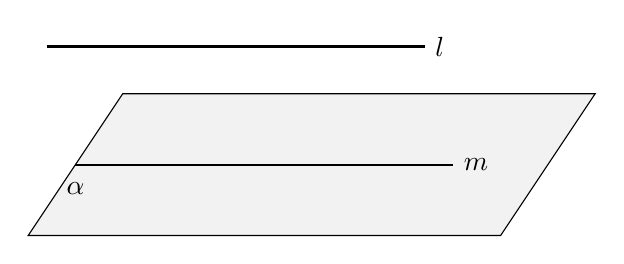
\begin{tikzpicture}[scale=1.2]
        % 绘制平面 alpha
        \draw[fill=gray!10] (0,0) -- (5,0) -- (6,1.5) -- (1,1.5) -- cycle;
        \node at (0.5, 0.5) {$\alpha$};

        % 绘制平面内的直线 m
        \draw[thick] (0.5, 0.75) -- (4.5, 0.75) node[right]{$m$};

        % 绘制平面外的直线 l
        \draw[thick] (0.2, 2) -- (4.2, 2) node[right]{$l$};
    \end{tikzpicture}
\end{center}

% --- 性质定理 2 ---
\begin{theorem}
    如果一条直线与一个平面平行，则过这条直线的任一平面与此平面的交线与该直线平行。
    \begin{equation*}
        \left.
        \begin{array}{l}
            l \parallel \alpha, l \subset \beta \\
            \alpha \cap \beta = m
        \end{array}
        \right\} \implies l \parallel m
    \end{equation*}
\end{theorem}
\begin{center}
    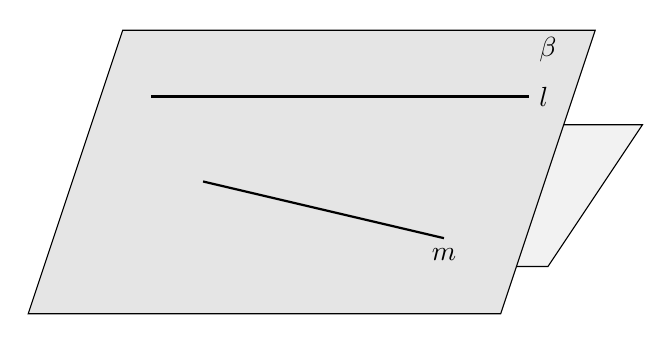
\begin{tikzpicture}[scale=1.2]
        % 绘制平面 alpha
        \draw[fill=gray!10] (0,0) -- (5,0) -- (6,1.5) -- (1,1.5) -- cycle;
        \node at (0.5, 0.3) {$\alpha$};

        % 绘制平面 beta
        \draw[fill=gray!20] (0.5, 2.5) -- (5.5, 2.5) -- (4.5, -0.5) -- (-0.5, -0.5) -- cycle;
        \node at (5, 2.3) {$\beta$};

        % 绘制直线 l
        \draw[thick] (0.8, 1.8) -- (4.8, 1.8) node[right]{$l$};

        % 绘制交线 m
        \draw[thick] (1.35, 0.9) -- (3.9, 0.3) node[below]{$m$};
    \end{tikzpicture}
\end{center}

\newpage

\section{线面垂直 (Line-Plane Perpendicular)}

% --- 判定定理 3 ---
\begin{theorem}
    如果一条直线与一个平面内的两条相交直线都垂直，那么该直线与此平面垂直。
    \begin{equation*}
        \left.
        \begin{array}{l}
            m \subset \alpha, n \subset \alpha, m \cap n = O \\
            l \perp m, l \perp n
        \end{array}
        \right\} \implies l \perp \alpha
    \end{equation*}
\end{theorem}
\begin{center}
    \begin{tikzpicture}[scale=1.2]
        % 绘制平面 alpha
        \draw[fill=gray!10] (0,0) -- (4,0) -- (5,1.5) -- (1,1.5) -- cycle;
        \node at (0.5, 0.4) {$\alpha$};

        % 定义交点O
        \coordinate (O) at (2.5, 0.75);

        % 绘制平面内的两条相交直线
        \draw[thick] (1,0.25) -- (4.5,1.45) node[right]{$n$};
        \draw[thick] (0.5,1.35) -- (4,0.3) node[right]{$m$};
        \fill (O) circle (1.5pt) node[below left]{$O$};

        % 绘制垂线 l
        \draw[thick] (2.5,-0.5) -- (2.5, 2) node[above]{$l$};

        % 标记垂直
        \draw (O) -- (O -| {$(2.2, 0.75)$}) -- (O -| {$(2.2, 1)$});
        \draw (O) -- (O -| {$(2.8, 0.75)$}) -- (O -| {$(2.8, 0.9)$});
    \end{tikzpicture}
\end{center}

% --- 性质定理 3 ---
\begin{theorem}
    垂直于同一个平面的两条直线平行。
    \begin{equation*}
        \left.
        \begin{array}{l}
            l \perp \alpha \\
            m \perp \alpha
        \end{array}
        \right\} \implies l \parallel m
    \end{equation*}
\end{theorem}
\begin{center}
    \begin{tikzpicture}[scale=1.2]
        % 绘制平面 alpha (与线线平行的性质图一致)
        \draw[fill=gray!10] (0,0) -- (4,0) -- (5,1.5) -- (1,1.5) -- cycle;
        \node at (0.5, 0.4) {$\alpha$};

        % 绘制直线 l
        \draw[thick] (2, -0.5) -- (2, 2.5) node[above]{$l$};
        \coordinate (O1) at (2,0.75);

        % 绘制直线 m
        \draw[thick] (3.5, -0.5) -- (3.5, 2.5) node[above]{$m$};
        \coordinate (O2) at (3.5, 0.5);

        % 标记 l 垂直于平面
        \draw (O1) -- (O1 -| {$(2.3, 0.75)$}) -- (O1 -| {$(2.3, 0.6)$});

        % 标记 m 垂直于平面
        \draw (O2) -- (O2 -| {$(3.8, 0.5)$}) -- (O2 -| {$(3.8, 0.35)$});
    \end{tikzpicture}
\end{center}

\newpage

\section{面面垂直 (Plane-Plane Perpendicular)}

% --- 判定定理 4 ---
\begin{theorem}
    如果一个平面经过另一个平面的一条垂线，那么这两个平面互相垂直。
    \begin{equation*}
        \left.
        \begin{array}{l}
            l \subset \beta \\
            l \perp \alpha
        \end{array}
        \right\} \implies \alpha \perp \beta
    \end{equation*}
\end{theorem}
\begin{center}
    \begin{tikzpicture}[scale=1.2]
        % 绘制平面 alpha
        \draw[fill=gray!10] (0,0) -- (4,0) -- (5,1.5) -- (1,1.5) -- cycle;
        \node at (0.5, 0.4) {$\alpha$};

        % 绘制平面 beta
        \coordinate (A) at (2.5, -0.5);
        \coordinate (B) at (2.5, 2);
        \coordinate (C) at (4.5, 2.5);
        \coordinate (D) at (4.5, 0);
        \draw[fill=gray!20] (A) -- (B) -- (C) -- (D) -- cycle;
        \node at (4.3, 2.2) {$\beta$};

        % 绘制垂线 l
        \draw[thick] (A) -- (B) node[above right]{$l$};

        % 标记垂直
        \coordinate (O) at (2.5, 0.75);
        \draw (O) -- (O -| {$(2.8, 0.75)$}) -- (O -| {$(2.8, 0.6)$});
    \end{tikzpicture}
\end{center}

% --- 性质定理 4 ---
\begin{theorem}
    如果两个平面互相垂直，那么在一个平面内垂直于它们交线的直线垂直于另一个平面。
    \begin{equation*}
        \left.
        \begin{array}{l}
            \alpha \perp \beta, \alpha \cap \beta = l \\
            m \subset \alpha, m \perp l
        \end{array}
        \right\} \implies m \perp \beta
    \end{equation*}
\end{theorem}
\begin{center}
    \begin{tikzpicture}[scale=1.2]
        % 绘制平面 beta (水平)
        \draw[fill=gray!10] (0,0) -- (5,0) -- (6,1.5) -- (1,1.5) -- cycle;
        \node at (0.5, 0.5) {$\beta$};

        % 绘制平面 alpha (垂直)
        \draw[fill=gray!20] (1.5,0.85) -- (4.5,0.25) -- (4.5,2.25) -- (1.5,2.85) -- cycle;
        \node at (1.7, 2.6) {$\alpha$};

        % 绘制交线 l
        \draw[thick] (1.5,0.85) -- (4.5,0.25) node[right]{$l$};

        % 绘制直线 m
        \coordinate (O) at (3, 0.55);
        \draw[thick] (O) -- (3, 2.55) node[above]{$m$};

        % 标记 m 垂直 l
        \draw (O) -- (O -| {$(2.7, 0.55)$}) -- (O -| {$(2.7, 0.75)$});
    \end{tikzpicture}
\end{center}

\subsection{证明线面平行}

\begin{example}
    如图，$A B C D$ 是边长为3的正方形，$D E \perp$ 平面 $A B C D, ~ A F / / D E$ 且 $D E=2 A F=4$ ．
    \begin{enumerate}
        \item 求证：$B F / /$ 平面 $D E C$ ；
        \item 求平面 $B E C$ 与平面 $B E F$ 夹角的余弦值；
        \item 求点 $D$ 到平面 $B E F$ 的距离.
    \end{enumerate}
\end{example}

\begin{figure} [H]
    \centering
    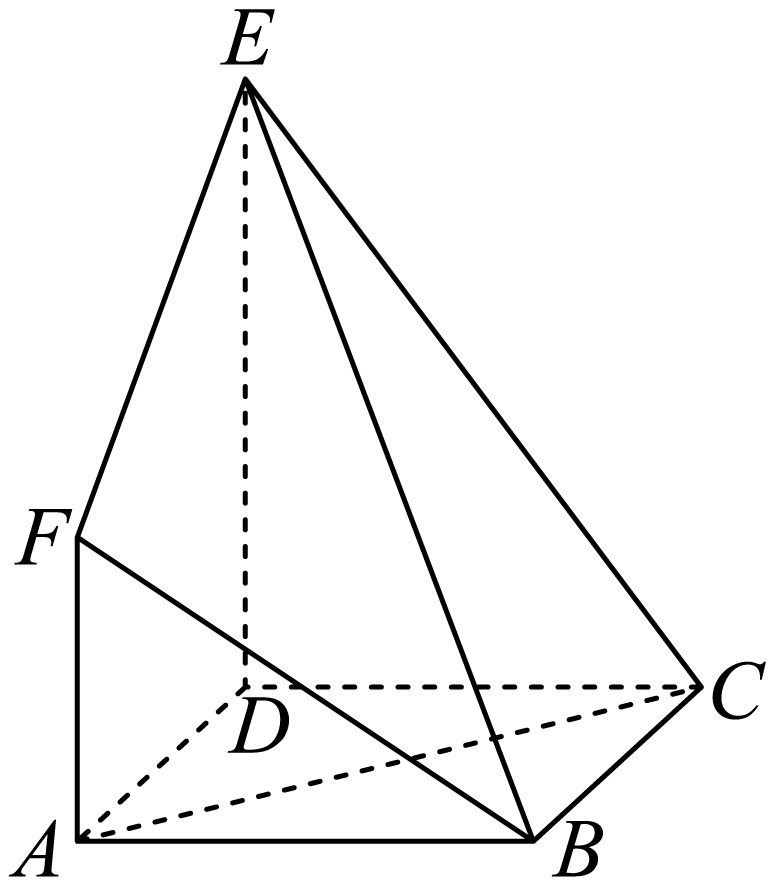
\includegraphics[width=0.2\textwidth]{chapters/立体几何/images/立体几何的几何法证明/img-20250824212921.png}
\end{figure}

\begin{example}
    如图，四棱锥 $P-A B C D$ 中，$P D \perp D A, P D \perp D C$ ，在底面 $A B C D$ 中，$A B \| D C, ~ A B \perp A D$ ，且 $2 A B=C D=6$ ， $A D=P D=4, ~ E$ 为 $P C$ 的中点．
    \begin{enumerate}
        \item 求证：$B E / /$ 平面 $A D P$ ；
        \item 求异面直线 $P A$ 与 $B C$ 所成的角的余弦值．
    \end{enumerate}
\end{example}

\begin{figure} [H]
    \centering
    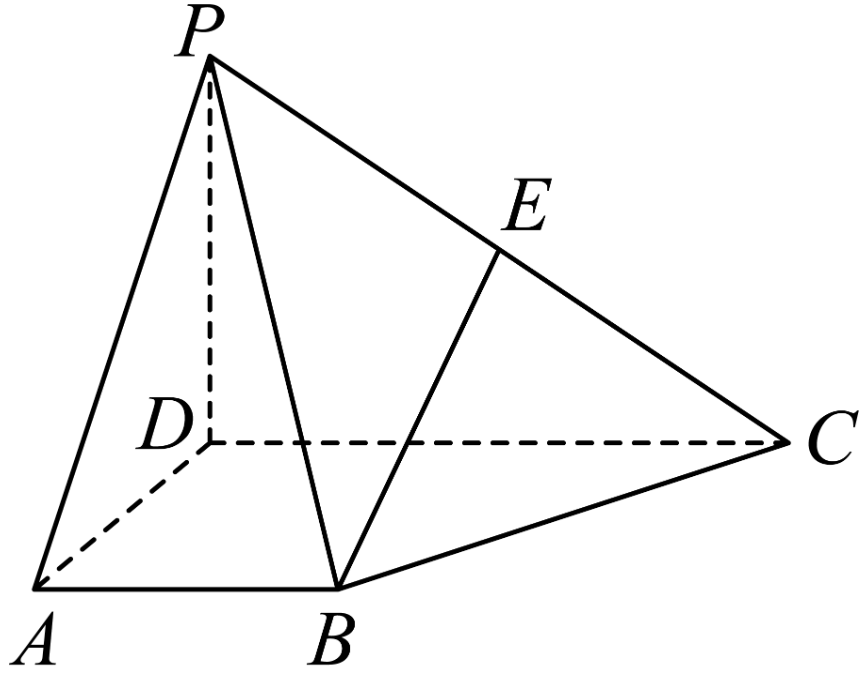
\includegraphics[width=0.2\textwidth]{chapters/立体几何/images/立体几何的几何法证明/img-20250824213020.png}
\end{figure}

\subsection{证明线线垂直}

\begin{theorem}[线面垂直的性质]

\end{theorem}

\begin{example}
    如图，四棱雉 $S-A B C D$ 的底面是边长为 2 的正方形，每条侧棱的长都是底面边长的 $\sqrt{2}$ 倍，$P$ 为侧棱 $S D$ 上的点，且 $S B / /$ 平面 $P A C$ ．
    \begin{enumerate}
        \item 求证：$A C \perp S D$ ．

        \item 求直线 $S B$ 到平面 $P A C$ 的距离．

        \item 请判断在平面 $P A C$ 上是否存在一点 $E$ ，使得 $\triangle E S B$ 是以 $S B$ 为底边，$\frac{2 \pi}{3}$ 为顶角的等腰三角形．若存在，请求出点 $E$ 的轨迹；若不存在，请说明理由．
    \end{enumerate}
\end{example}

\begin{figure} [H]
    \centering
    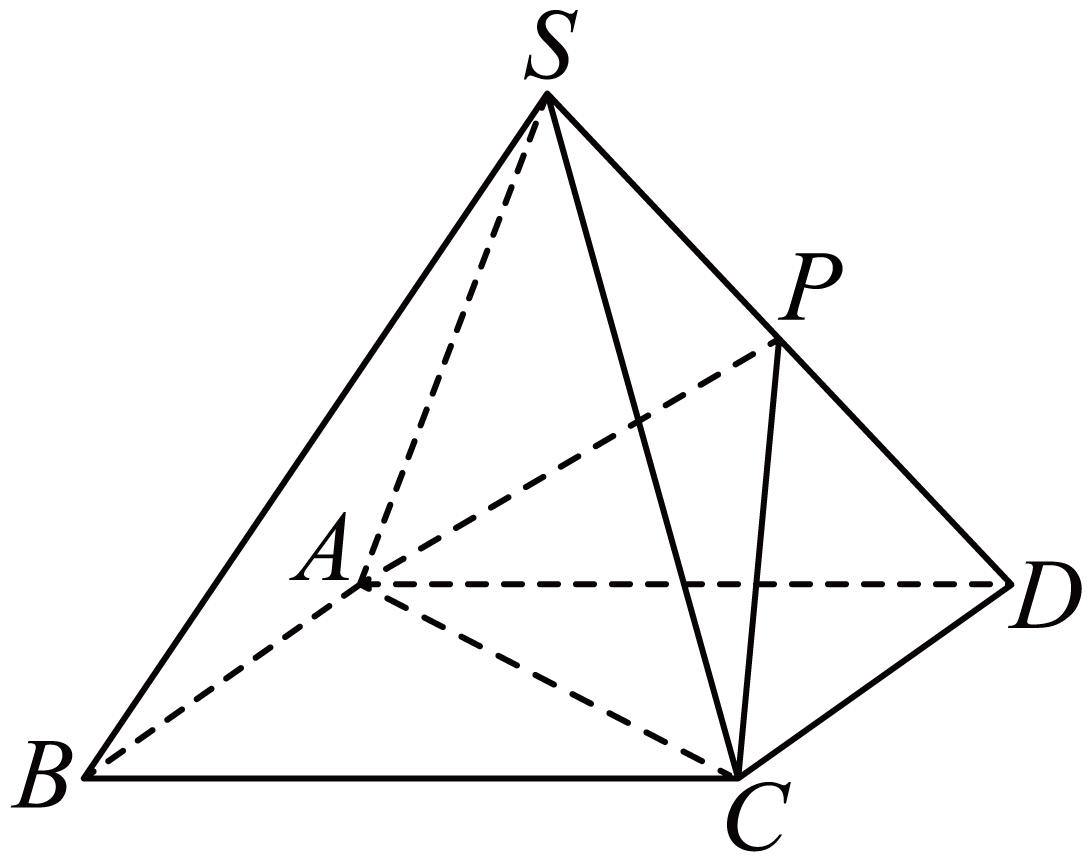
\includegraphics[width=0.2\textwidth]{chapters/立体几何/images/立体几何的几何法证明/img-20250824213613.png}
\end{figure}

\section{证明线面垂直}

\begin{example}
    底面为菱形的四棱雉 $P-A B C D$ 中，$A C$ 与 $B D$ 交于点 $O$ ，平面 $P B D \perp$ 平面 $A B C D$ ，平面 $P A C \perp$ 平面 $A B C D$ ．
    \begin{enumerate}
        \item 证明：$P O \perp$ 平面 $A B C D$ ；

        \item 若 $O A=2 O D=2$ ，直线 $D C$ 与平面 $P B C$ 所成角的正弦值为 $\frac{4 \sqrt{5}}{15}$ ，求平面 $P A C$ 与平面 $P B C$ 夹角的余弦值．
    \end{enumerate}
\end{example}

\begin{figure} [H]
    \centering
    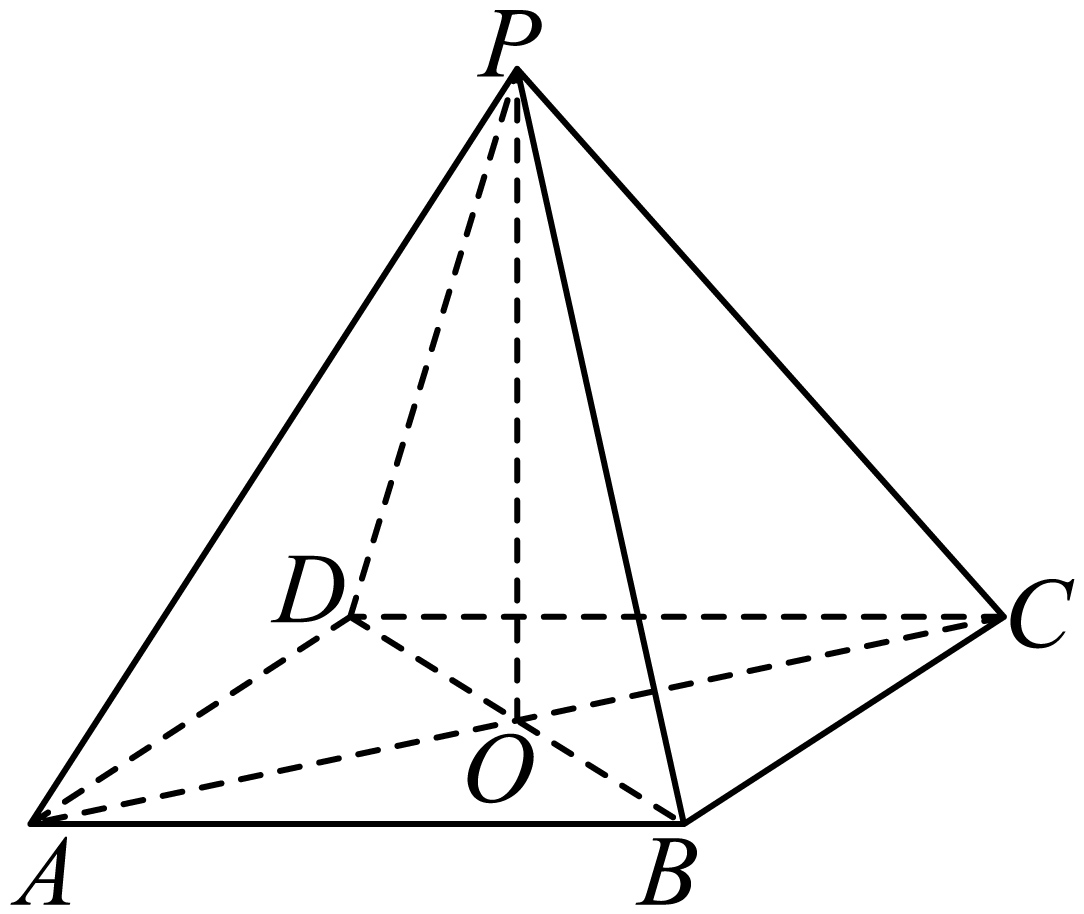
\includegraphics[width=0.2\textwidth]{chapters/立体几何/images/立体几何的几何法证明/img-20250824213654.png}
\end{figure}
